\documentclass[a4paper, 11pt, uplatex]{jsarticle}
\usepackage{amsmath, amssymb}
\usepackage{bm}
\usepackage[dvipdfmx]{graphicx}
\usepackage{here}
\usepackage{multirow}

%テキストの表示領域の調節
\setlength{\textwidth}{\paperwidth}
\addtolength{\textwidth}{-40truemm}
\setlength{\textheight}{\paperheight}
\addtolength{\textheight}{-45truemm}

%余白の調節
\setlength{\topmargin}{-10.4truemm}
\setlength{\evensidemargin}{-5.4truemm}
\setlength{\oddsidemargin}{-5.4truemm}
\setlength{\headheight}{17pt}
\setlength{\headsep}{10mm}
\addtolength{\headsep}{-17pt}
\setlength{\footskip}{5mm}

% \nofiles
\begin{document}
\section{目的}
コンピュータをはじめ, NC工作機械, 家電製品等にはディジタル回路が多用されている.
そこで, 実際に広く用いられているディジタル用ICを用いて, 論理回路の基礎的事項について実験し, ディジタル回路の使い方,
ディジタル回路の動作, ディジタル回路の設計法を学ぶ.
\section{実験方法}
実験にはサンハヤト社製のIC実験・応用セットICトレーナー(MODELCT-311S),
ACアダプタ, およびCT-311S用実習セット(MODEL  CT-311S-P01)から構成される実験装置を用いた.
この装置のブレッドボード上にIC, 抵抗, コンデンサなどの回路素子を固定してリード線で結線し,
以下の7個の回路を作成し,  動作を実際に確認した.
\begin{itemize}
  \item 2入力EX-OR回路
  \item 2入力4出力デコーダ(解読器)
  \item ハーフ・アダー(全加算器)
  \item Dラッチ回路
  \item J-Kフリップフロップ
  \item Dフリップフロップを用いた1/2分周器
  \item 非同期16進カウンタ
\end{itemize}

\section{実験項目}
\subsection{ゲート回路のまとめ(基本素子6種類)}
レポート末尾に一覧表を添付した.
\subsection{2入力EX-ORゲート}
\subsubsection{2入力EX-ORゲート}

作成した2入力EX-ORゲートの回路図を図\ref{EX-OR}に示す.
また,  実験から得られたEX-OR回路の動作表を表\ref{EX-OR動作表}に,  EX-OR機能の真理値表を表\ref{EX-OR真理値表}に示す.
ここで, 図\ref{EX-OR}の回路図から2入力EX-OR回路の論理式を求める.
図\ref{EX-OR}の点3, 11, 6をそれぞれ$\mathrm{C_1}, \mathrm{C_2}, \mathrm{C_3}$とする.

\begin{align}
  \mathrm{C_1} &= \overline{\mathrm{A} \cdot \mathrm{B}} \\
  \mathrm{C_2} &= \overline{(\overline{\mathrm{A} \cdot \mathrm{B}}) \cdot \mathrm{B}} = (\mathrm{A} \cdot \mathrm{B}) + \overline{\mathrm{B}}\\
  \mathrm{C_3} &= \overline{(\overline{\mathrm{A} \cdot \mathrm{B}}) \cdot \mathrm{A}} = (\mathrm{A} \cdot \mathrm{B}) + \overline{\mathrm{A}}\\
  \mathrm{Y} &= \overline{\mathrm{C_2} \cdot \mathrm{C_3}}
             = (\overline{\mathrm{A} \cdot \mathrm{B}}) \cdot \mathrm{B} + (\overline{\mathrm{A} \cdot \mathrm{B}}) \cdot \mathrm{A}
             = (\overline{\mathrm{A}} + \overline{\mathrm{B}}) \cdot \mathrm{B} + (\overline{\mathrm{A}} + \overline{\mathrm{B}}) \cdot \mathrm{A}\\
             &= (\overline{\mathrm{A}} + \overline{\mathrm{B}}) \cdot (\mathrm{A} + \mathrm{B}) = \mathrm{A} \cdot \overline{\mathrm{B}} + \overline{\mathrm{A}} \cdot  \mathrm{B} \\
             &= \mathrm{A} \oplus \mathrm{B}
\end{align}


\begin{figure}[H]
  \begin{center}
    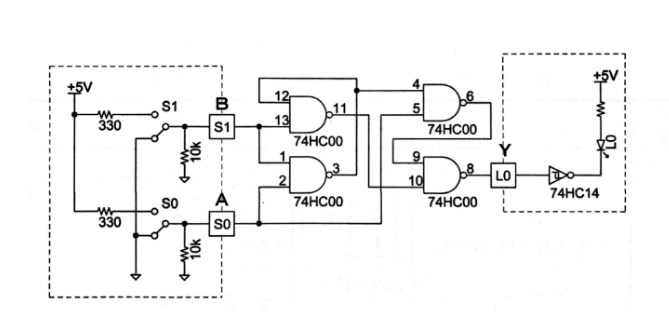
\includegraphics[width = 8cm]{画像/EX-OR.png}
    \caption{NAND素子4個を用いたEX-OR機能の回路図}
    \label{EX-OR}
  \end{center}
\end{figure}

\begin{table}[H]
  \begin{center}
  \caption{EX-OR回路の動作表}
  \label{EX-OR動作表}
\begin{tabular}{|l|l|l|l|}
\hline
                    & \multicolumn{2}{l|}{入力} & 出力 \\ \hline
接続端子               & S0         & S1         & L0 \\ \hline
端子名                 & A          & B          & Y  \\ \hline \hline
\multirow{4}{*}{電圧} & L          & L          & L  \\
                     & L          & H          & H  \\
                     & H          & L          & H  \\
                     & H          & H          & L  \\ \hline
\end{tabular}
\end{center}
\end{table}

\begin{table}[H]
  \begin{center}
  \caption{EX-OR機能の真理値表}
  \label{EX-OR真理値表}
\begin{tabular}{|l|l|l|l|}
\hline
                    & \multicolumn{2}{l|}{入力} & 出力 \\ \hline
端子名                 & A          & B          & Y  \\ \hline \hline
\multirow{4}{*}{真理値} & 0          & 0          & 0 \\
                      & 0          & 1          & 1 \\
                      & 1          & 0          & 1 \\
                      & 1          & 1          & 0  \\ \hline
\end{tabular}
\end{center}
\end{table}

実験より, S0, S1の入力不一致の時にのみL0のLEDが点灯し, Hを出力するのを確認することができた.
また,  2入力が一致しているときはLEDがつかないことも確認し, EX-OR機能について理解することができた.

\subsubsection{課題:実験で作成した2入力EX-OR回路を正論理/負論理のNAND素子を使って書き換える}
実験ではNAND素子を4個使用して2入力EX-OR回路を作成したが,  ここでは正論理/負論理のNAND素子を使用する.
すると, 以下の図\ref{EX-OR書き換え}のような回路によって書き換えられる.
\begin{figure}[H]
  \begin{center}
    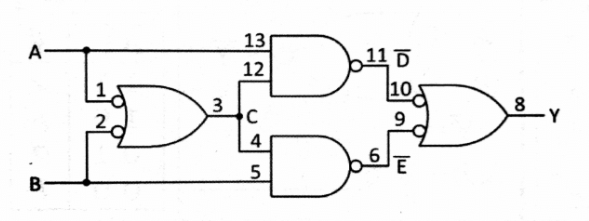
\includegraphics[width = 8cm]{画像/EX-OR書き換え.png}
    \caption{正論理/負論理のNAND素子を用いたEX-OR機能の回路図}
    \label{EX-OR書き換え}
  \end{center}
\end{figure}

この回路のC, $\overline{\mathrm{D}}$, $\overline{\mathrm{E}}$においての論理式は以下のようになる.
\begin{align}
  \mathrm{C} &= \overline{\mathrm{A}} + \overline{\mathrm{B}} \\
  \overline{\mathrm{D}} & = \mathrm{A} \cdot (\overline{\mathrm{A}} + \overline{\mathrm{B}})
  = \mathrm{A} \cdot \overline{\mathrm{A}} + \mathrm{A} \cdot \overline{\mathrm{B}} = \mathrm{A} \cdot \overline{\mathrm{B}}\\
  \overline{\mathrm{E}} &= \mathrm{B} \cdot \mathrm{C} = \mathrm{B} \cdot (\overline{\mathrm{A}} + \overline{\mathrm{B}})
  \\ &= \overline{\mathrm{A}} \cdot \mathrm{B}
\end{align}
よって, この回路の出力Yの論理式は, 次のようになる.
\begin{align}
  \mathrm{Y} &= \overline{\mathrm{D}} + \overline{\mathrm{E}} = \mathrm{A} \cdot \overline{\mathrm{B}} + \overline{\mathrm{A}} \cdot \mathrm{B}
  \\ &= \mathrm{A} \oplus \mathrm{B}
\end{align}
以上より,  図\ref{EX-OR書き換え}に示す回路は2入力EX-OR回路の機能を持つことがわかる.

\subsection{デコーダとエンコーダ}
\subsubsection{デコーダ}
デコーダ回路は,  2桁の2進数をスイッチ(S1, S0)を使って入力し,  10進数の0から3を表すLED(L0〜L3)に"1(H)"を出力する,  すなわち対応するLEDが点灯する回路である.

\par

実験により作成した2入力4出力デコーダを図\ref{デコーダ}に示す.
また,  実験から得られたデコーダの動作表を表\ref{デコーダ動作表}に,  EX-OR機能の真理値表を表\ref{デコーダ真理値表}に示す.

\begin{figure}[H]
  \begin{center}
    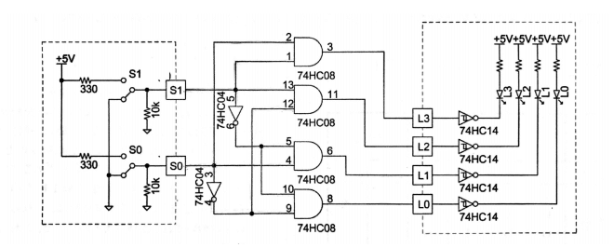
\includegraphics[width = 8cm]{画像/デコーダ.png}
    \caption{2入力4出力デコーダの回路図}
    \label{デコーダ}
  \end{center}
\end{figure}

\begin{table}[H]
  \begin{center}
  \caption{デコーダの動作表}
  \label{デコーダ動作表}
\begin{tabular}{|c|c|c|c|c|c|c|}
\hline
                    & \multicolumn{2}{c|}{入力} & \multicolumn{4}{c|}{出力} \\ \hline
端子名                &S1 & S0 &L0 &L1 &L2 &L3  \\ \hline \hline
\multirow{4}{*}{電圧} & L & L &H &L &L &L \\
                     & L & H &L &H &L &L \\
                     & H & L &L &L &H &L \\
                     & H & H &L &L &L &H \\ \hline
\end{tabular}
\end{center}
\end{table}

\begin{table}[H]
  \begin{center}
  \caption{デコーダの真理値表}
  \label{デコーダ真理値表}
\begin{tabular}{|c|c|c|c|c|c|c|}
\hline
                    & \multicolumn{2}{c|}{入力} & \multicolumn{4}{c|}{出力} \\ \hline
端子名                &S1 & S0 &L0 &L1 &L2 &L3  \\ \hline \hline
\multirow{4}{*}{真理値} & 0 & 0 &1 &0 &0 &0 \\
                     & 0 & 1 &0 &1 &0 &0 \\
                     & 1 & 0 &0 &0 &1 &0 \\
                     & 1 & 1 &0 &0 &0 &1 \\ \hline
\end{tabular}
\end{center}
\end{table}

表\ref{デコーダ真理値表}の真理値表からデコーダの論理式は以下のようになる.
\begin{align}
  \mathrm{L0} &= \overline{\mathrm{S0}} \cdot \overline{\mathrm{S1}} \\
  \mathrm{L1} &= \mathrm{S0} \cdot \overline{\mathrm{S1}} \\
  \mathrm{L2} &= \overline{\mathrm{S0}} \cdot \mathrm{S1} \\
  \mathrm{L3} &= \mathrm{S0} \cdot \mathrm{S1}
\end{align}

このデコーダ回路は, 2桁の2進数を入力すると,  それに対応する10進数を出力する回路である.
具体的には,  S1が2進数の上位ビット,  S0が2進数の下位ビットを表し,  L0〜L3はそれぞれ10進数の0〜3を表す.
確かに(S1, S0) = (0, 0), (0, 1), (1, 0), (1, 1)はそれぞれL0〜L3(0〜3)に対応していることが真理値表から分かる.
つまり2桁2進数で入力されたものをデコーダ回路が解読して10進数に変換して出力していることが確認できる.

\subsubsection{課題:4入力2出力エンコーダ回路の設計}
エンコーダ(符号変換器)は,  10進数を2進数に変換する回路である.
今回の課題では,  10進数0から3をそれぞれに対応する4つのスイッチ(S0, S1, S2, S3)を用いて入力し,
2つのLED$(\mathrm{L1} ,  \mathrm{L0})$を用いて2ビットの2進数を出力するエンコーダ回路を設計し,  作成した.

\par
4入力2出力エンコーダの真理値表を表\ref{エンコーダ真理値表}に示す.
\begin{table}[H]
  \begin{center}
  \caption{エンコーダの真理値表}
  \label{エンコーダ真理値表}
\begin{tabular}{|c|c|c|c|c|c|c|}
\hline
                    & \multicolumn{4}{l|}{入力} & \multicolumn{2}{l|}{出力} \\ \hline
端子名                &S0 & S1 &S2 &S3 &L1 &L0  \\ \hline \hline
\multirow{4}{*}{真理値} & 1 & 0 &0 &0 &0 &0 \\
                     & 0 & 1 &0 &0 &0 &1 \\
                     & 0 & 0 &1 &0 &1 &0 \\
                     & 0 & 0 &0 &1 &1 &1 \\ \hline
\end{tabular}
\end{center}
\end{table}

表\ref{エンコーダ真理値表}の真理値表からエンコーダの論理式は以下のようになる.
\begin{align}
  \mathrm{L0} &= \mathrm{S1} + \mathrm{S3} \\
  \mathrm{L1} &= \mathrm{S2} + \mathrm{S3}
\end{align}

論理式から回路を設計すると以下の回路図(図\ref{エンコーダ})のようになった.

\begin{figure}[H]
  \begin{center}
    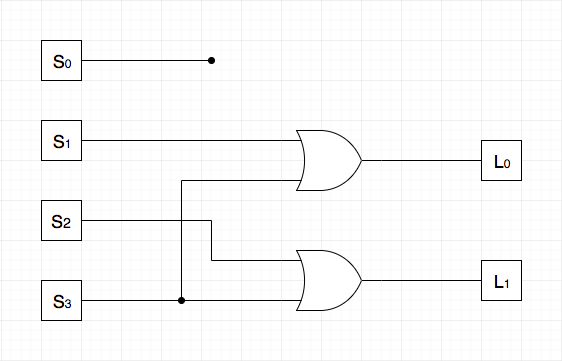
\includegraphics[width = 8cm]{画像/エンコーダ.png}
    \caption{4入力2出力エンコーダの回路図}
    \label{エンコーダ}
  \end{center}
\end{figure}

\subsection{加算回路}
\subsubsection{ハーフ・アダー}
ハーフ・アダー(半加算器)は,  2進数の足し算,  具体的には2つの入力AとBを加算し,  その和S(Sum)と桁上げC(Carry)を出力する.

ハーフアダーの真理値表は次の表\ref{ハーフアダー真理値表}の通りである.
\begin{table}[H]
  \begin{center}
  \caption{ハーフ・アダーの真理値表}
  \label{ハーフアダー真理値表}
\begin{tabular}{|c|c|c|c|c|}
  \hline
                      & \multicolumn{2}{l|}{\multirow{2}{*}{入力}} & \multicolumn{2}{l|}{出力} \\ \cline{4-5}
                      & \multicolumn{2}{l|}{}                    & 和          & 桁上げ        \\ \hline
  端子名                 & A                   & B                  & S          & C          \\ \hline \hline
  \multirow{4}{*}{真理値} & 0                   & 0                  & 0          & 0          \\
                      & 0                   & 1                  & 1          & 0          \\
                      & 1                   & 0                  & 1          & 0          \\
                      & 1                   & 1                  & 0          & 1          \\ \hline
\end{tabular}
\end{center}
\end{table}

真理値表から論理式を導くと以下のようになる.
\begin{align}
  \mathrm{S} &= \overline{\mathrm{A}} \cdot \mathrm{B} + \mathrm{A} \cdot \overline{\mathrm{B}} \\ &= \mathrm{A} \oplus \mathrm{B} \\
  \mathrm{C} &= \mathrm{A} \cdot \mathrm{B}
\end{align}

また,  ハーフ・アダーの回路図を以下の図\ref{ハーフアダー}に示す.
\begin{figure}[H]
  \begin{center}
    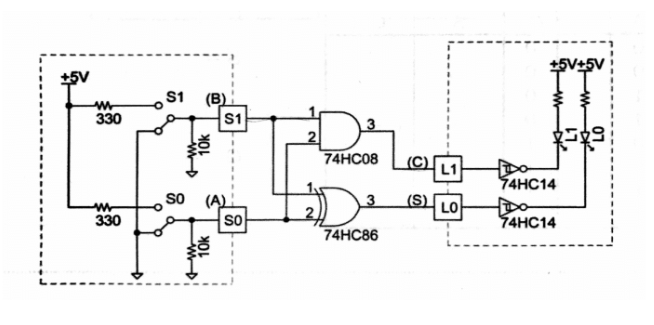
\includegraphics[width = 8cm]{画像/ハーフアダー.png}
    \caption{ハーフ・アダーの回路図}
    \label{ハーフアダー}
  \end{center}
\end{figure}

ハーフ・アダー回路を実際に作成し,  動作確認をすると,  次の動作表(表\ref{ハーフアダー動作表})が得られた.

\begin{table}[H]
  \begin{center}
  \caption{ハーフ・アダーの動作表}
  \label{ハーフアダー動作表}
\begin{tabular}{|c|c|c|c|c|}
  \hline
                      & \multicolumn{2}{l|}{\multirow{2}{*}{入力}} & \multicolumn{2}{l|}{出力} \\ \cline{4-5}
                      & \multicolumn{2}{l|}{}                    & 和          & 桁上げ        \\ \hline
  接続端子                & S0                  & S1                 & L0         & L1         \\ \hline
  端子名                 & A                   & B                  & S          & C          \\ \hline \hline
  \multirow{4}{*}{電圧} & L                   & L                  & L          & L          \\
                      & L                   & H                  & H          & L          \\
                      & H                   & L                  & H          & L          \\
                      & H                   & H                  & L          & H          \\ \hline
\end{tabular}
\end{center}
\end{table}

真理値表と動作表を比較すると,  Hと1,  Lと0が全て対応しているため,  今回作成したハーフ・アダーが正常に機能していることが確認できた.
また,  真理値表及び論理式から,  1桁同士の2進数の加算の和はEX-OR機能で表現でき,  桁上げはAND機能で表現できることが分かった.

\subsubsection{課題1:フル・アダー}
フル・アダー回路は2進数の足し算に加え(A,  B),  桁上げによる入力($\mathrm{C_{in}}$)の3入力を加算し,  その和Sと桁上げ$\mathrm{C_{out}}$を出力する.

フル・アダー回路の真理値表を以下の表\ref{フルアダー真理値表}に示す.
\begin{table}[H]
  \begin{center}
  \caption{フル・アダーの真理値表}
  \label{フルアダー真理値表}
\begin{tabular}{|c|c|c|c|c|c|}
  \hline
                      & \multicolumn{3}{l|}{\multirow{2}{*}{入力}} & \multicolumn{2}{l|}{出力} \\ \cline{5-6}
                      & \multicolumn{3}{l|}{}                    & 和          & 桁上げ        \\ \hline
  端子名                 & A         & B        &$\mathrm{C_{in}}$       & S        & $\mathrm{C_{out}}$          \\ \hline \hline
  \multirow{8}{*}{真理値} & 0          &0         & 0          & 0      &0   \\
                       & 0          &1         & 0          & 1      &0    \\
                       & 1          &0         & 0          & 1      &0    \\
                       & 1          &1         & 0          & 0      &1    \\
                       & 0          &0         & 1          & 1      &0    \\
                       & 0          &1         &1           &0       &1    \\
                       & 1          &0         &1           &0       &1    \\
                       & 1          &1         &1           &1       &1    \\ \hline
\end{tabular}
\end{center}
\end{table}

真理値表から論理式を導くと次のようになる.
\begin{align}
  \mathrm{S} &= (\overline{\mathrm{A}} \cdot \overline{\mathrm{B}} \cdot \mathrm{C_{in}})
   + (\overline{\mathrm{A}} \cdot \mathrm{B} \cdot \overline{\mathrm{C_{in}}})
   + (\mathrm{A} \cdot \overline{\mathrm{B}} \cdot \overline{\mathrm{C_{in}}})
   + (\mathrm{A} \cdot \mathrm{B} \cdot \mathrm{C_{in}}) \\
   &= (\overline{\mathrm{A}} \cdot \overline{\mathrm{B}} + \mathrm{A} \cdot \mathrm{B}) \cdot \mathrm{C_{in}} + (\overline{\mathrm{A}} \cdot \mathrm{B} + \mathrm{A} \cdot \overline{\mathrm{B}}) \cdot \overline{\mathrm{C_{in}}}  \\
   &= (\overline{\overline{\mathrm{A}} \cdot \mathrm{B} + \mathrm{A} \cdot \overline{\mathrm{B}}}) \cdot \mathrm{C_{in}} + (\overline{\mathrm{A}} \cdot \mathrm{B} + \mathrm{A} \cdot \overline{\mathrm{B}}) \cdot \overline{\mathrm{C_{in}}} \\
   &= (\mathrm{A} \oplus \mathrm{B}) \oplus \mathrm{C_{in}} \\
  \mathrm{\mathrm{C_{out}}} &= (\mathrm{A} \cdot \mathrm{B} \cdot \overline{\mathrm{C_{in}}})
  + (\overline{\mathrm{A}} \cdot \mathrm{B} \cdot \mathrm{C_{in}})
  + (\mathrm{A} \cdot \overline{\mathrm{B}} \cdot \mathrm{C_{in}})
  + (\mathrm{A} \cdot \mathrm{B} \cdot \mathrm{C_{in}}) \\
   &= (\mathrm{A} \cdot \mathrm{B}) \cdot (\mathrm{C_{in}} + \overline{\mathrm{C_{in}}}) + (\overline{\mathrm{A}} \cdot \mathrm{B} + \mathrm{A} \cdot \overline{\mathrm{B}}) \cdot \mathrm{C_{in}}\\
   &=\mathrm{A} \cdot \mathrm{B} + (\mathrm{A} \oplus \mathrm{B}) \cdot \mathrm{C_{in}}
\end{align}

またフル・アダーの回路図を以下の図\ref{フルアダー}に示す.
\begin{figure}[H]
  \begin{center}
    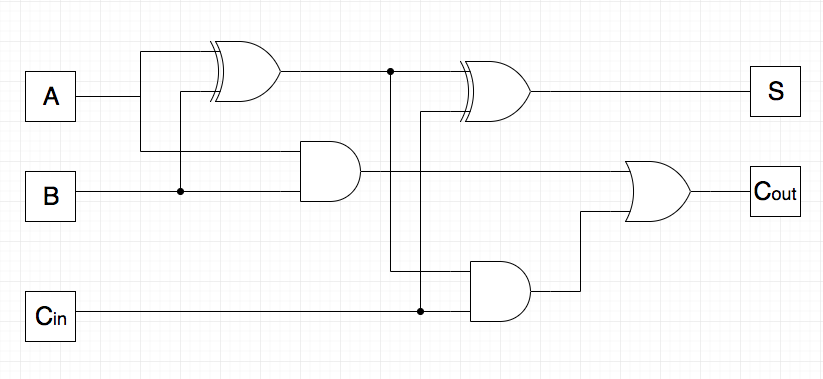
\includegraphics[width = 8cm]{画像/フルアダー.png}
    \caption{フル・アダーの回路図}
    \label{フルアダー}
  \end{center}
\end{figure}

\subsubsection{課題2:2桁の2進数の加算回路}
2桁の2進数同士の加算を可能にする加算回路をする. 具体的な手順としては1桁目の加算を行い,  桁上げと和を出力する.
次に桁上げされた入力と2桁目を加算し,  桁上げと和を出力する. 1桁目の加算ではハーフ・アダー回路を用い,  2桁目の加算ではフル・アダー回路を用いることで
2桁の2進数の加算回路が実現される.

2桁の2進数の加算回路の真理値表を表\ref{加算回路真理値表}に示す.
3.4.1,3.4.2節で求めた論理式を用いると, 2桁の2進数の加算回路の論理式は以下のようになる.

\begin{align}
  \mathrm{S0} &= \mathrm{A0} \oplus \mathrm{B0} \\
  \mathrm{C1} &= \mathrm{A0} \cdot \mathrm{B0} \\
  \mathrm{S1} &= (\mathrm{A1} \oplus \mathrm{B1}) \oplus \mathrm{C1} \\
              &= (\mathrm{A1} \oplus \mathrm{B1}) \oplus (\mathrm{A0} \cdot \mathrm{B0})\\
  \mathrm{C2} &= \mathrm{A1} \cdot \mathrm{B1} + (\mathrm{A1} \oplus \mathrm{B1}) \cdot \mathrm{C1} \\
              &= (\mathrm{A1} \cdot \mathrm{B1}) + (\mathrm{A1} \oplus \mathrm{B1}) \cdot (\mathrm{A0} \cdot \mathrm{B0}) \\
\end{align}

\begin{table}[H]
\begin{center}
\caption{2桁の2進数の加算回路の真理値表}
\label{加算回路真理値表}
\begin{tabular}{|l|l|l|l|l|l|l|l|}
\hline
                      & \multicolumn{4}{l|}{\multirow{2}{*}{入力}} & \multicolumn{3}{l|}{出力} \\ \cline{6-8}
                      & \multicolumn{4}{l|}{}                    & 3桁目    & 2桁目    & 1桁目   \\ \hline
端子名                   & A1       & A0       & B1       & B0      & C2     & C1     & C0    \\ \hline \hline
\multirow{16}{*}{真理値} & 0        & 0        & 0        & 0       & 0      & 0      & 0     \\
                      & 0        & 1        & 0        & 0       & 0      & 0      & 1     \\
                      & 1        & 0        & 0        & 0       & 0      & 1      & 0     \\
                      & 1        & 1        & 0        & 0       & 0      & 1      & 1     \\
                      & 0        & 0        & 0        & 1       & 0      & 0      & 1     \\
                      & 0        & 1        & 0        & 1       & 0      & 1      & 0     \\
                      & 1        & 0        & 0        & 1       & 0      & 1      & 1     \\
                      & 1        & 1        & 0        & 1       & 1      & 0      & 0     \\
                      & 0        & 0        & 1        & 0       & 0      & 1      & 0     \\
                      & 0        & 1        & 1        & 0       & 0      & 1      & 1     \\
                      & 1        & 0        & 1        & 0       & 1      & 0      & 0     \\
                      & 1        & 1        & 1        & 0       & 1      & 0      & 1     \\
                      & 0        & 0        & 1        & 1       & 0      & 1      & 1     \\
                      & 0        & 1        & 1        & 1       & 1      & 0      & 0     \\
                      & 1        & 0        & 1        & 1       & 1      & 0      & 1     \\
                      & 1        & 1        & 1        & 1       & 1      & 1      & 0     \\ \hline
\end{tabular}
\end{center}
\end{table}

\begin{figure}[H]
  \begin{center}
    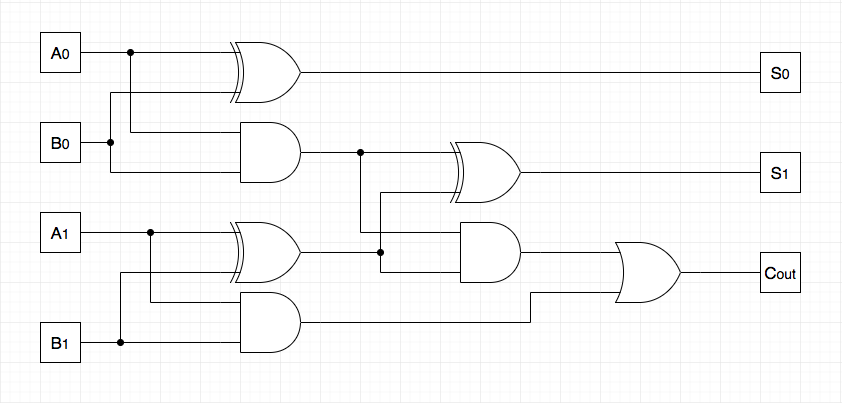
\includegraphics[width = 8cm]{画像/加算回路.png}
    \caption{2桁の2進数の加算回路図}
    \label{加算回路}
  \end{center}
\end{figure}


\subsection{Dラッチ回路}

Dラッチ回路の回路図を以下の図\ref{Dラッチ}に示す.

\begin{figure}[H]
  \begin{center}
    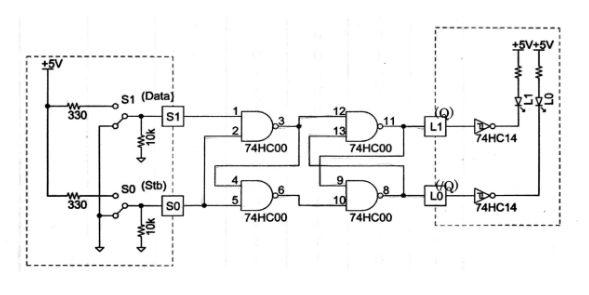
\includegraphics[width = 8cm]{画像/Dラッチ.png}
    \caption{Dラッチの回路図}
    \label{Dラッチ}
  \end{center}
\end{figure}

また,  実験によって確認したDラッチの動作表(表\ref{Dラッチ動作表})とDラッチのタイムチャート(図\ref{Dラッチタイムチャート})を以下に示す.

\begin{table}[H]
  \begin{center}
  \caption{Dラッチの動作表}
  \label{Dラッチ動作表}
\begin{tabular}{|l|l|l|l|l|}
\hline
                    & \multicolumn{2}{l|}{入力} & \multicolumn{2}{l|}{出力}  \\ \hline
接続端子               & S1         & S0         & L1    &L0\\ \hline
端子名                 & Data          & $\overline{\mathrm{Std}}$          &Q     &$\overline{\mathrm{Q}}$\\ \hline \hline
\multirow{4}{*}{電圧} & L          & L          &Q0      &$\overline{\mathrm{Q0}}$\\
                     & H          & L          &Q0      &$\overline{\mathrm{Q0}}$\\
                     & L          & H          &L      &H  \\
                     & H          & H          &H      &L  \\ \hline
\end{tabular}
\end{center}
\end{table}

\begin{figure}[H]
  \begin{center}
    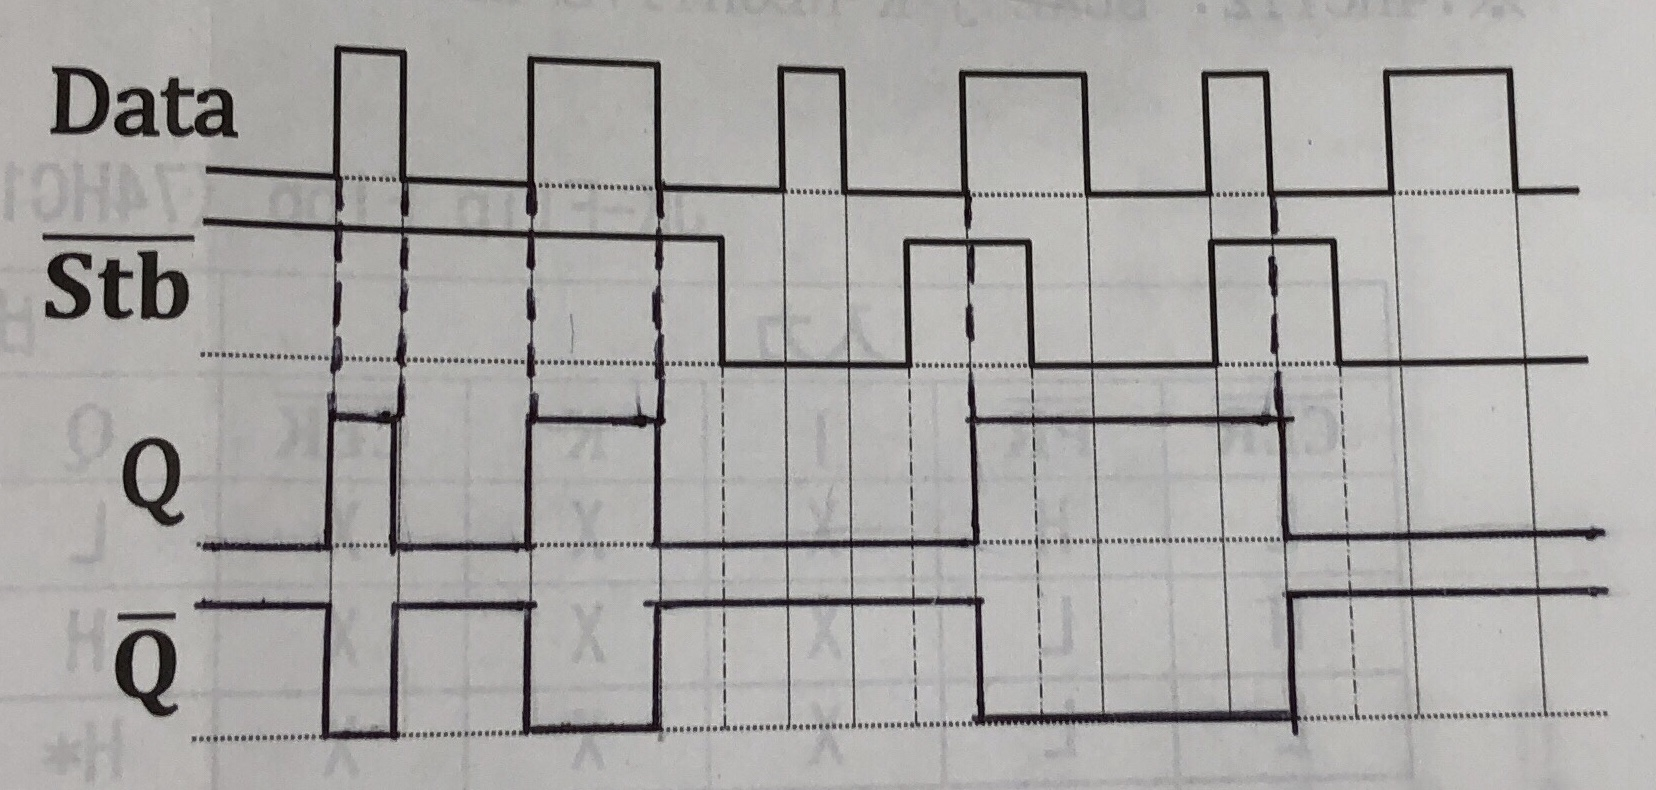
\includegraphics[width = 8cm]{画像/Dラッチタイムチャート.jpg}
    \caption{Dラッチのタイムチャート}
    \label{Dラッチタイムチャート}
  \end{center}
\end{figure}

Dラッチの動作表からDラッチ回路の機能を考察する.
ストローブ信号がHの時,  出力QはDataがLならLを出力し,  HならHを出力する,  つまり入力されたDataと同じ信号を出力している. 
ストローブ信号がLの時には,  出力QはQ0, つまり直前の出力Qの信号を出力する.
\par
次に,  これらの機能をタイムチャートを参照しながら確かめる.最初はストローブ信号がHであり,  DataとQの信号が一致している.
Data, QがともにLの状態でストローブ信号をLにしたのち,  DataをL→H→Lと入力してもQはLのままであった.
再びストローブをHに戻し,  DataにHを入力するとQもHを出力した.

以上の動きから,  ストローブ信号の機能はHであるときには入力信号をそのまま出力し, Lにしたときには直前の出力を保持する機能であることがわかった.
また, ラッチ機能とはある時点での出力を保持し続け, 記憶しておく機能のことである.

\subsection{フリップフロップ回路}
\subsubsection{J-Kフリップフロップ}

J-Kフリップフロップの回路図を以下の図\ref{JK}に示す.

\begin{figure}[H]
  \begin{center}
    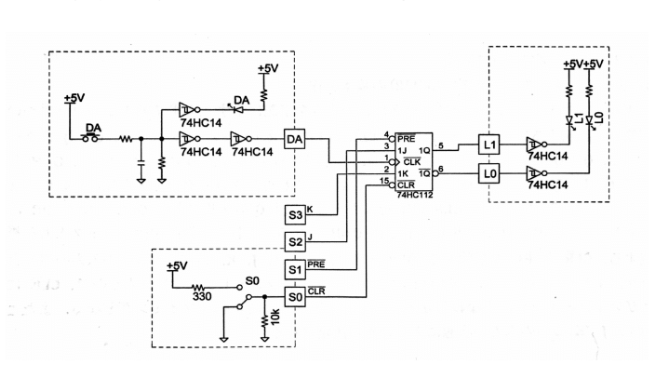
\includegraphics[width = 8cm]{画像/JK回路図.png}
    \caption{J-Kフリップフロップの回路図}
    \label{JK}
  \end{center}
\end{figure}

また,  実験によって確認したJ-Kフリップフロップの動作表(表\ref{JK動作表})とタイムチャート(図\ref{JKタイムチャート})を以下に示す.

\begin{table}[H]
  \begin{center}
    \caption{J-Kフリップフロップの動作表}
    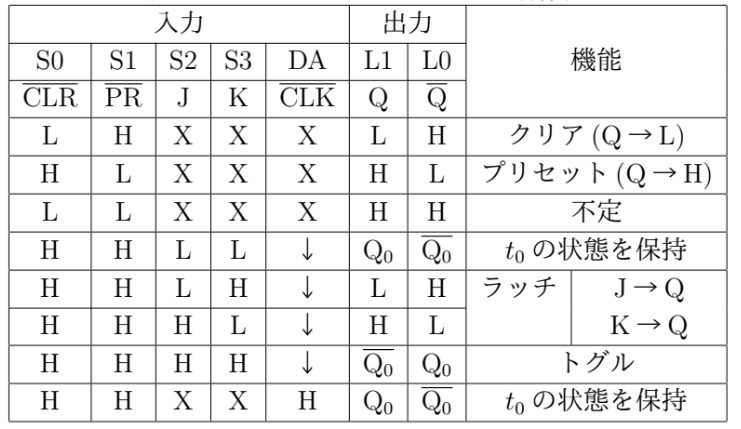
\includegraphics[width = 8cm]{画像/JK動作表.png}
    \label{JK動作表}
  \end{center}
\end{table}

\begin{figure}[H]
  \begin{center}
    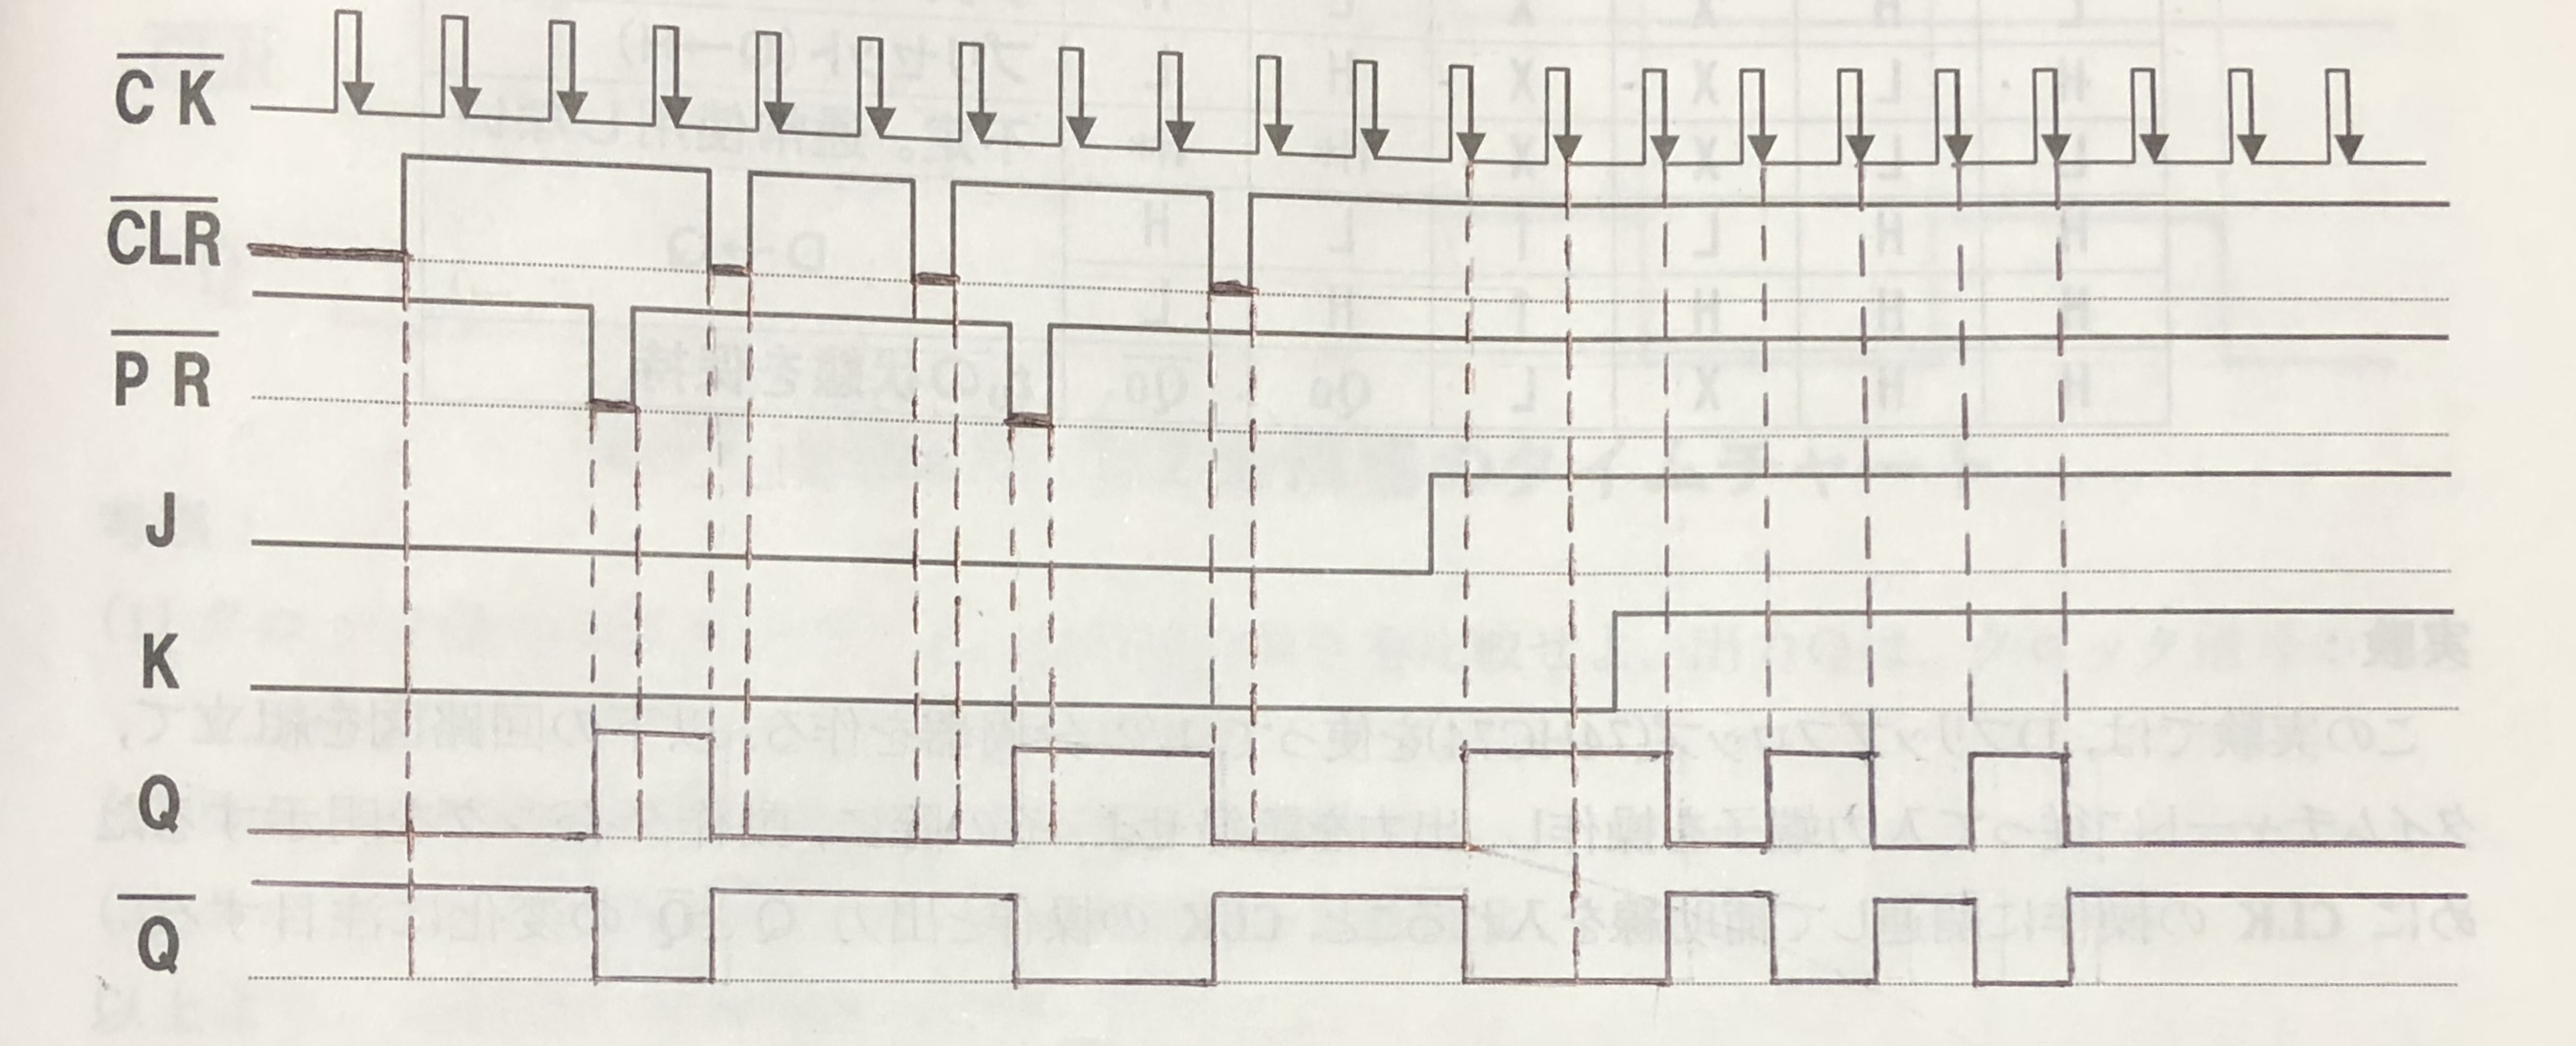
\includegraphics[width = 8cm]{画像/JKタイムチャート.jpg}
    \caption{J-Kフリップフロップのタイムチャート}
    \label{JKタイムチャート}
  \end{center}
\end{figure}

まずタイムチャートの前半部分から,  $\overline{\mathrm{CLK}},  \overline{\mathrm{PR}}$の操作と出力Qの変化に注目して考察する.
$\overline{\mathrm{CLR}}$をLからHにしても変化はなく, $\overline{\mathrm{PR}}$がHからLになった時点でQがLからHに変化している.
に,  $\overline{\mathrm{PR}}$をLからHにしても変化はなく, $\overline{\mathrm{CLR}}$がHからLになった時点でQがHからLに変化している.
しかしながら,  QがLの状態で$\overline{\mathrm{CLR}}$をHからLにしてもQはLのままであった.
これらの信号の変化から,  $\overline{\mathrm{CLR}}$と$\overline{\mathrm{PR}}$はクロック信号とは関係なく動作し,
$\overline{\mathrm{CLR}}$にLを入力するとQをLに変化させ,  $\overline{\mathrm{PR}}$にLを入力すると,  QをHに変化させる働きがあることがわかった.
\par
次にタイムチャートの後半部分から,  J, Kの状態と$\overline{\mathrm{CLK}}$の操作と出力Qの変化を考察する.
JがH,  KがL,  QがLの状態の時,  $\overline{\mathrm{CLK}}$が立ち下がった瞬間にQがHに変化している.
また,  J, Kが共にHの状態の時$\overline{\mathrm{CLK}}$が立ち下がるたびにQはHからLに,  またLからHに変化している.
以上のことから,  JがH, KがLの時には$\overline{\mathrm{CLK}}$が立ち下がる時にQをHに変化させ,
J,  Kが共にHの時には直前のQを反転させる, つまり$\overline{\mathrm{Q0}}$を出力するトグル機能をもつことがわかる.
また,  動作表を確認すると,  JがL, KがHの時には$\overline{\mathrm{CLK}}$が立ち下がった時にQをLに変化させることがわかる.

\subsubsection{Dフリップフロップを用いた分周器}

D-FFを用いた1/2分周器の回路図を以下の図\ref{Dフリップフロップ回路}に示す.

\begin{figure}[H]
  \begin{center}
    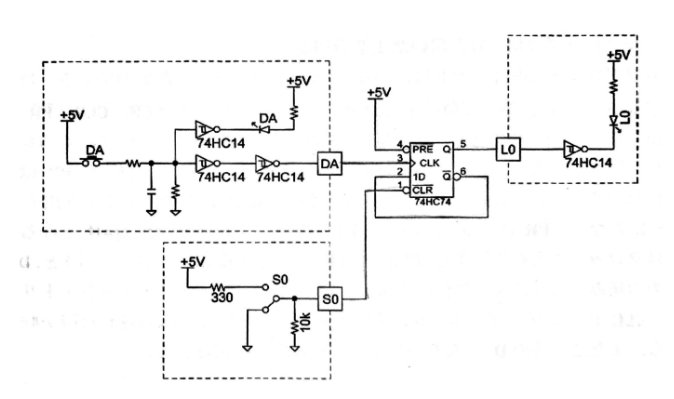
\includegraphics[width = 8cm]{画像/分周器.png}
    \caption{D-FFを用いた1/2分周器の回路図}
    \label{Dフリップフロップ回路}
  \end{center}
\end{figure}

また,  実験によって確認したJ-Kフリップフロップの動作表(表\ref{DFF動作表})とタイムチャート(図\ref{DFFタイムチャート})を以下に示す.

\begin{table}[H]
  \begin{center}
    \caption{D-FFを用いた1/2分周器の動作表}
    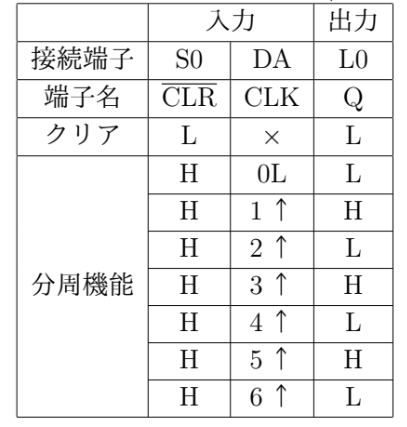
\includegraphics[width = 8cm]{画像/DFF動作表.png}
    \label{DFF動作表}
  \end{center}
\end{table}

\begin{figure}[H]
  \begin{center}
    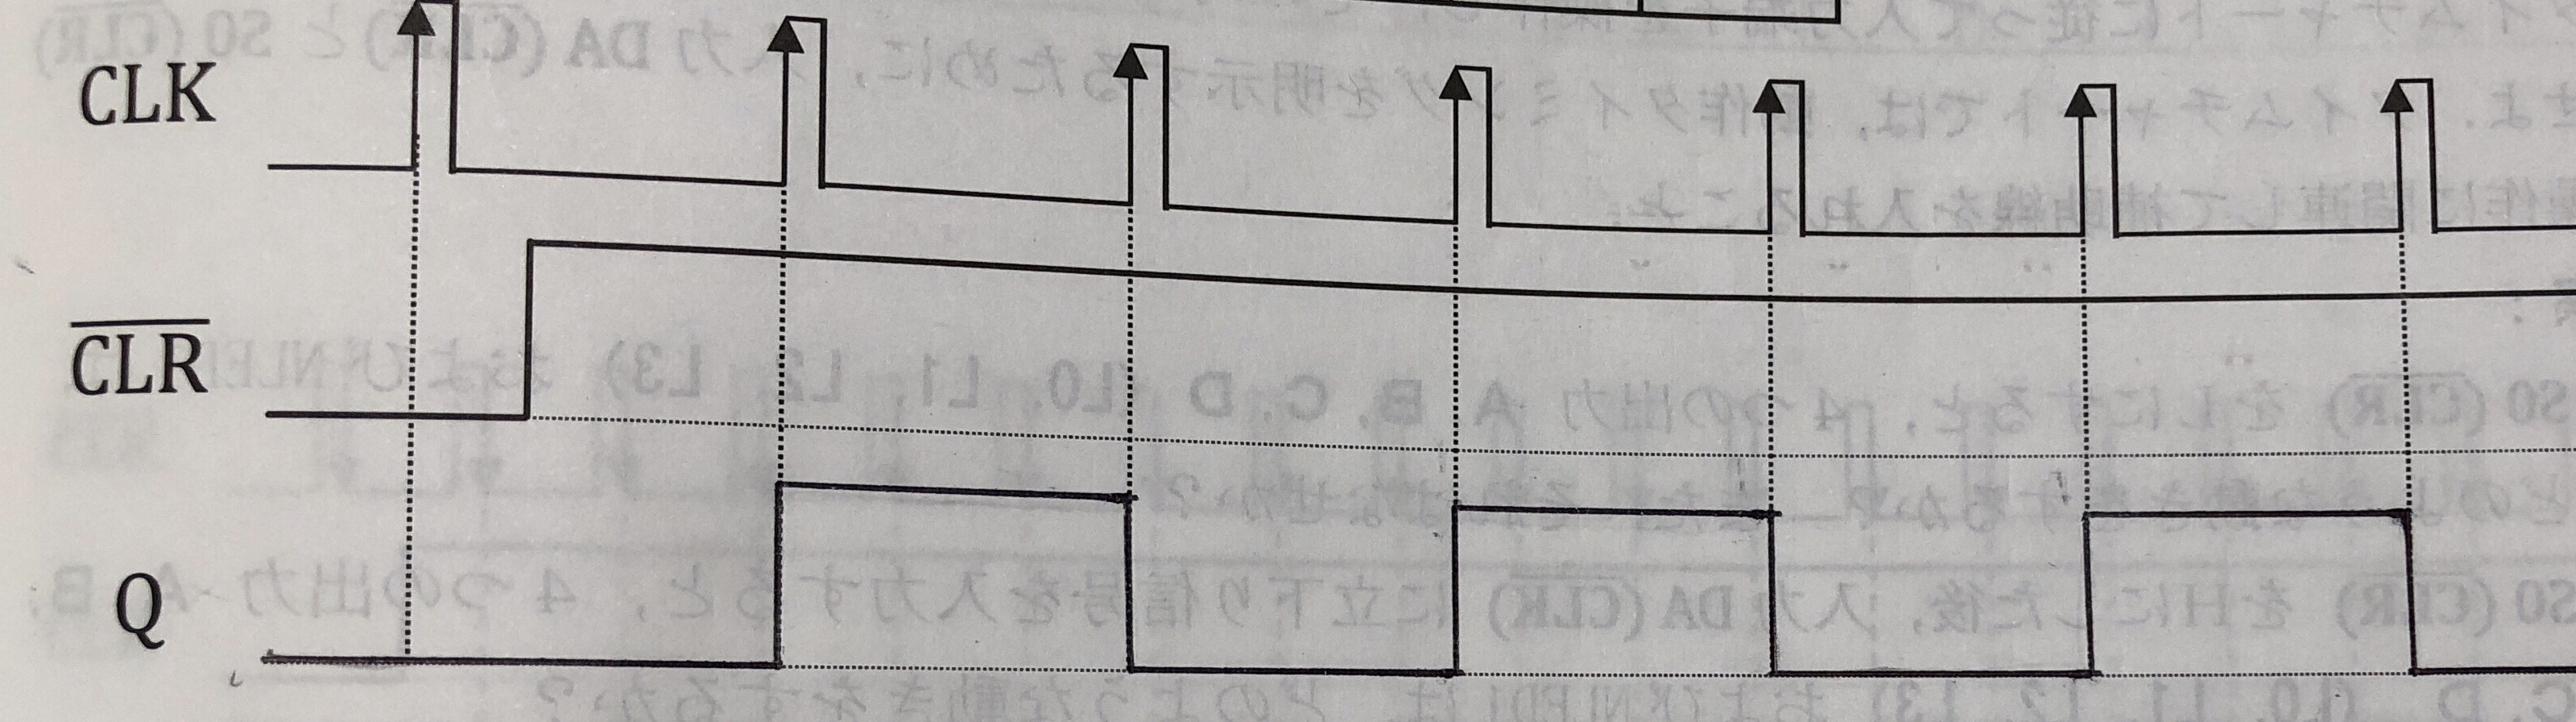
\includegraphics[width = 8cm]{画像/DFFタイムチャート.jpg}
    \caption{D-FFを用いた1/2分周器のタイムチャート}
    \label{DFFタイムチャート}
  \end{center}
\end{figure}

タイムチャートから分周器の機能を考察する.
$\overline{\mathrm{CLR}}$がLの状態ではCLKが立ち上がってもQに変化はない.
$\overline{\mathrm{CLR}}$がHの状態ではCLKが立ち上がるたびにQがHからLに,  LからHに変化させるトグル機能であることがわかる.
QがLから再びLに戻るまでにCLKが2回立ち上がっていることがわかる,  つまりCLKの周期をTとするとQの周期は2Tとなる.
そのため,  周波数はCLKの周波数は$f_{\mathrm{CLK}}=1/T$であり,  Qの周波数は$f_\mathrm{Q}=1/2T=f_{\mathrm{CLK}}/2$となる.
つまり,  分周器の分周機能とは,  入力された信号の周波数を落として出力する(今回は1/2倍にした)機能である.

\subsection{カウンタ回路}

非同期16進カウンタの回路図を以下の図\ref{カウンタ回路}に示す.

\begin{figure}[H]
  \begin{center}
    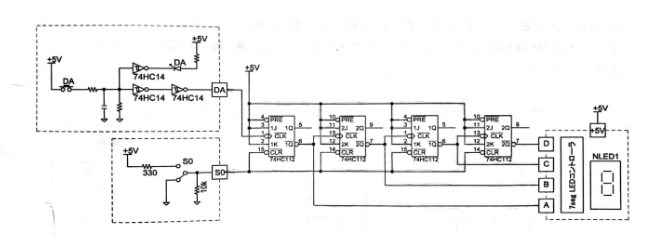
\includegraphics[width = 8cm]{画像/カウンタ.png}
    \caption{非同期16進数カウンタの回路図}
    \label{カウンタ回路}
  \end{center}
\end{figure}

また,  実験によって確認した非同期16進カウンタの動作表(表\ref{カウンタ真理値表})とタイムチャート(図\ref{カウンタタイムチャート})を以下に示す.

\begin{table}[H]
  \begin{center}
  \caption{非同期16進カウンタの動作表}
  \label{カウンタ真理値表}
\begin{tabular}{|l|l|l|l|l|l|l|l|}
\hline
\multirow{2}{*}{\begin{tabular}[c]{@{}l@{}}$\overline{\mathrm{CLR}}$\\ S0\end{tabular}} & \multirow{2}{*}{\begin{tabular}[c]{@{}l@{}}$\overline{\mathrm{CLK}}$\\ DA\end{tabular}} & \multirow{2}{*}{\begin{tabular}[c]{@{}l@{}}D\\ L3\end{tabular}} & \multirow{2}{*}{\begin{tabular}[c]{@{}l@{}}C\\ L2\end{tabular}} & \multirow{2}{*}{\begin{tabular}[c]{@{}l@{}}B\\ L1\end{tabular}} & \multirow{2}{*}{\begin{tabular}[c]{@{}l@{}}A\\ L0\end{tabular}} & \multirow{2}{*}{\begin{tabular}[c]{@{}l@{}}NLED1\\ 7seg表示\end{tabular}} & \multirow{2}{*}{備考} \\
                                                                  &                                                                   &                                                                 &                                                                 &                                                                 &                                                                 &                                                                         &                     \\ \hline
L                                                                 & X                                                                 & H                                                               & H                                                               & H                                                               & H                                                               & F                                                                       & リセット                \\ \hline
H                                                                 & L                                                                 & H                                                               & H                                                               & H                                                               & H                                                               & F                                                                       & (15)                \\ \hline
H                                                                 & 1↓                                                                & L                                                               & L                                                               & L                                                               & L                                                               & 0                                                                       &                     \\ \hline
H                                                                 & 2↓                                                                & L                                                               & L                                                               & L                                                               & H                                                               & 1                                                                       &                     \\ \hline
H                                                                 & 3↓                                                                & L                                                               & L                                                               & H                                                               & L                                                               & 2                                                                       &                     \\ \hline
H                                                                 & 4↓                                                                & L                                                               & L                                                               & H                                                               & H                                                               & 3                                                                       &                     \\ \hline
H                                                                 & 5↓                                                                & L                                                               & H                                                               & L                                                               & L                                                               & 4                                                                       &                     \\ \hline
H                                                                 & 6↓                                                                & L                                                               & H                                                               & L                                                               & H                                                               & 5                                                                       &                     \\ \hline
H                                                                 & 7↓                                                                & L                                                               & H                                                               & H                                                               & L                                                               & 6                                                                       &                     \\ \hline
H                                                                 & 8↓                                                                & L                                                               & H                                                               & H                                                               & H                                                               & 7                                                                       &                     \\ \hline
H                                                                 & 9↓                                                                & H                                                               & L                                                               & L                                                               & L                                                               & 8                                                                       &                     \\ \hline
H                                                                 & 10↓                                                               & H                                                               & L                                                               & L                                                               & H                                                               & 9                                                                       &                     \\ \hline
H                                                                 & 11↓                                                               & H                                                               & L                                                               & H                                                               & L                                                               & A                                                                       &                     \\ \hline
H                                                                 & 12↓                                                               & H                                                               & L                                                               & H                                                               & H                                                               & b                                                                       &                     \\ \hline
H                                                                 & 13↓                                                               & H                                                               & H                                                               & L                                                               & L                                                               & C                                                                       &                     \\ \hline
H                                                                 & 14↓                                                               & H                                                               & H                                                               & L                                                               & H                                                               & d                                                                       &                     \\ \hline
H                                                                 & 15↓                                                               & H                                                               & H                                                               & H                                                               & L                                                               & E                                                                       &                     \\ \hline
H                                                                 & 16↓                                                               & H                                                               & H                                                               & H                                                               & H                                                               & F                                                                       &                     \\ \hline
H                                                                 & 17↓                                                               & L                                                               & L                                                               & L                                                               & L                                                               & 0                                                                       &                     \\ \hline
\end{tabular}
\end{center}
\end{table}

\begin{figure}[H]
  \begin{center}
    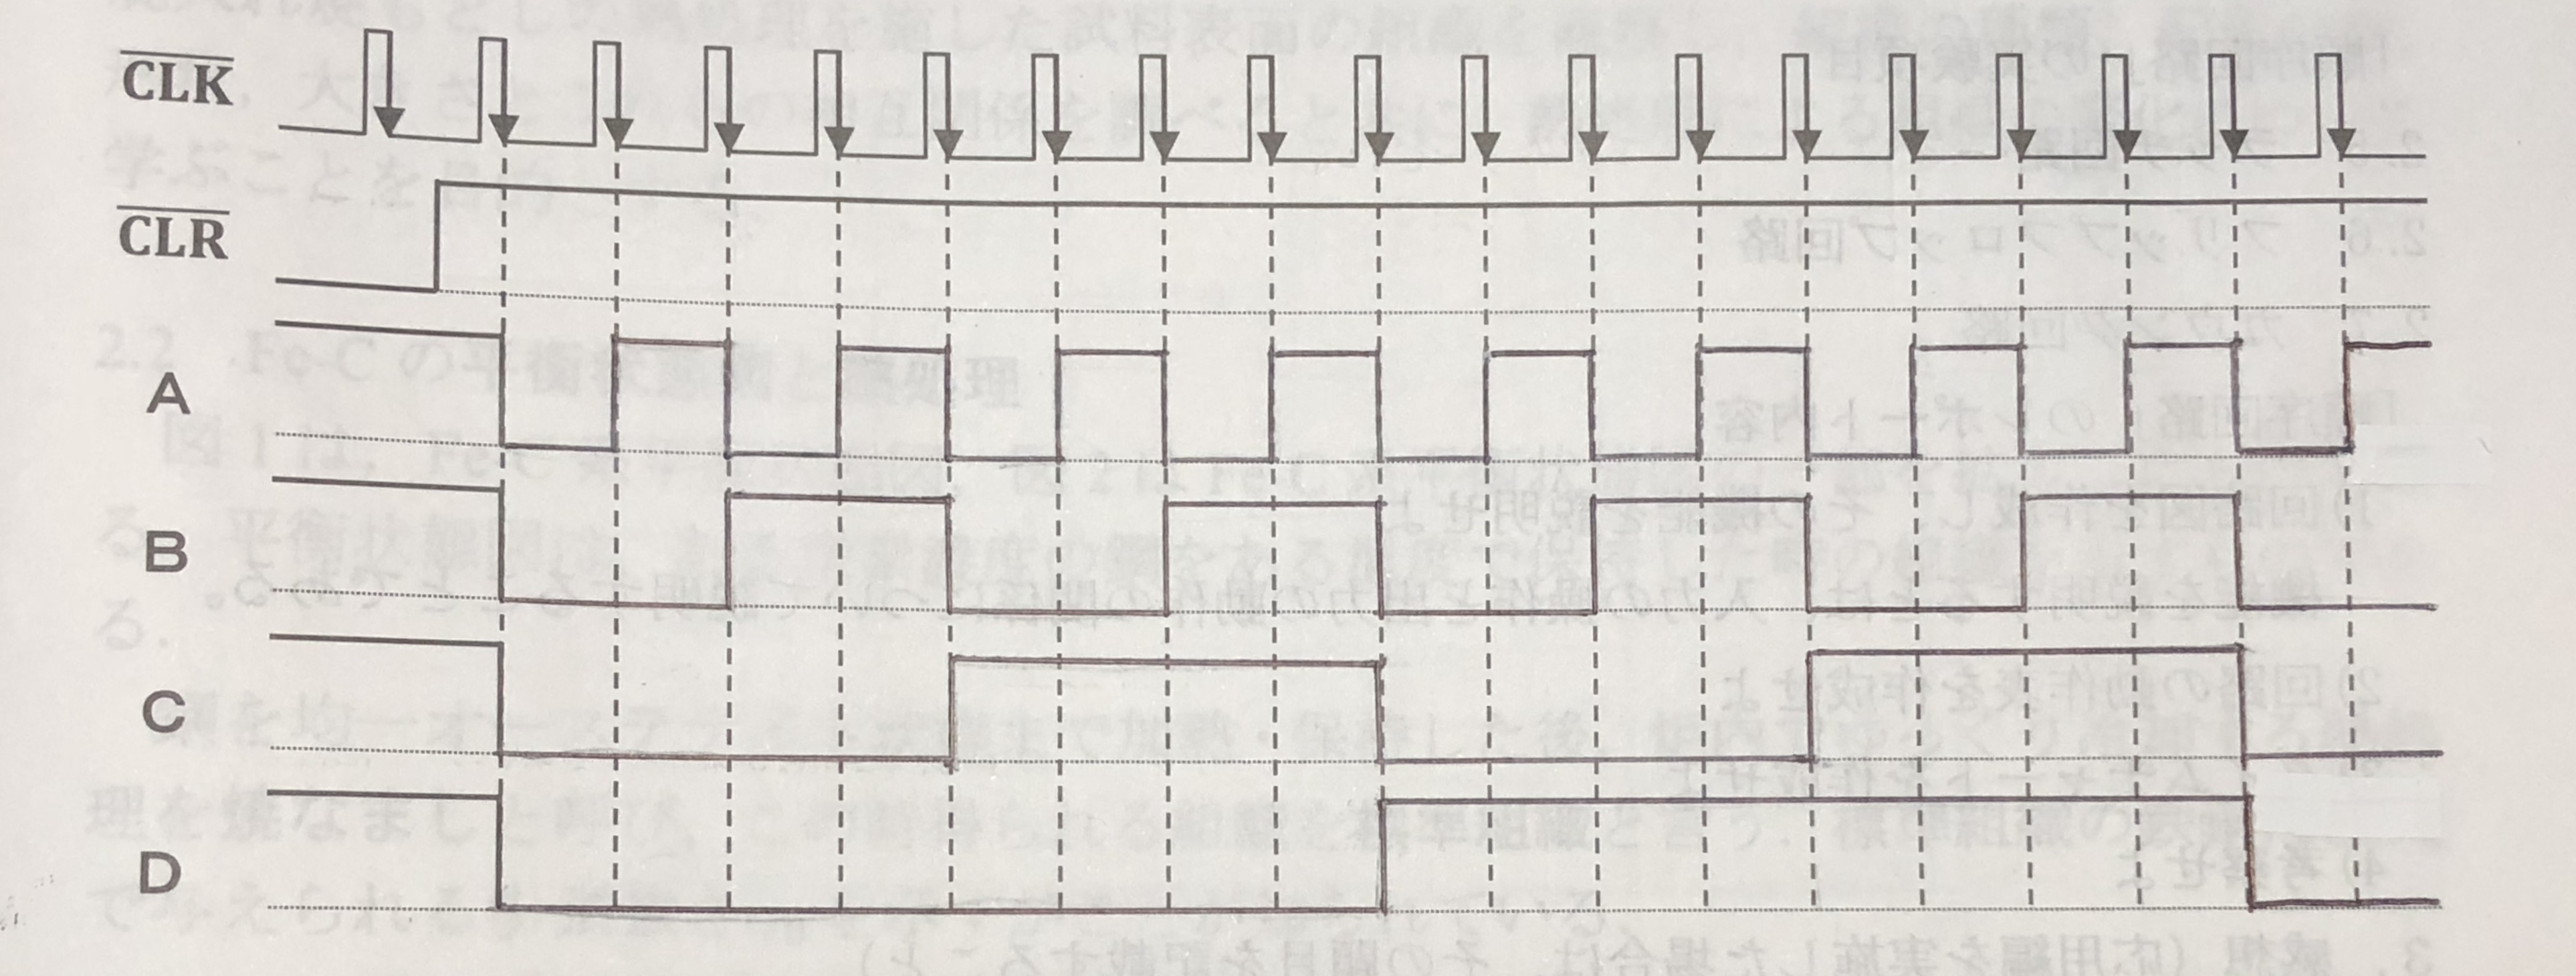
\includegraphics[width = 8cm]{画像/カウンタタイムチャート.jpg}
    \caption{非同期16進カウンタのタイムチャート}
    \label{カウンタタイムチャート}
  \end{center}
\end{figure}

$\overline{\mathrm{CLR}}$をLにすると4つの出力(ABCD)はHとなり,  NLED1にはFと表示された.
これは$\overline{\mathrm{CLR}}$をLにした時,  以前の状態に関わらずABCDをHにリセットするという役割があるためである.
次に,  $\overline{\mathrm{CLR}}$をHにし,  $\overline{\mathrm{CLK}}$に 立ち下がりを入力するとABCDがLに変化し,  NLED1には0が表示された
再び$\overline{\mathrm{CLK}}$に立ち下がりを入力するとAのみがHに変化し,  NLED1には1が表示された.
その後,  何度も立ち下がりを入力していくと,  AはL, Hを交互に繰り返し,  BはL, L, H, Hと2回ごとに,  Cは4回ごとに,  Dは8回ごとにLとHを入れ替えた.
NLED1は2,  3,  4,  \dots,  9,  A,  b,  C,  \dots,  Fと増加していき,  再び0に戻った.
DCBAと並び替え,  Hを1に,  Lを0に対応させると,  (0, 0, 0, 0), (0, 0, 0, 1), (0, 0, 1, 0), \dots,  (1, 1, 1, 0), (1, 1, 1, 1)のように増加している.
つまりDCBAは4桁の2進数を表しており,  ABCDはそれぞれ16進数の1, 2, 3, 4桁目, つまりそれぞれ$2^0, 2^1, 2^2, 2^3$を表しており,
$\mathrm{D} \times 2^3 + \mathrm{C} \times 2^2 + \mathrm{B} \times 2^1 + \mathrm{A} \times 2^0$を計算すると10進数表示することができる.
\par
続いて周期と周波数に着目する.
$\overline{\mathrm{CLK}}$の周期を$T$とすると, Aの周期は2$T$となっている.
また, Bの周期を$T_\mathrm{B}$とすると,  Cの周期は$2T_\mathrm{B}$,  Cの周期を$T_\mathrm{C}$とすると,  Dの周期は$2T_\mathrm{C}$とそれぞれ2倍になっている.
よってABCDの周期は$\overline{\mathrm{CLK}}$の周期を用いて,  2$T$,  4$T$,  8$T$,  16$T$となっている.
周波数も同様にして考えると,  Aの周波数は$T$の1/2倍,  Bの周波数はAの1/2倍,  Cの周波数はBの1/2倍,  Dの周波数はCの1/2倍である.
したがって,  $\overline{\mathrm{CLK}}$の周波数を$f$とするとABCDの周期はそれぞれ$1/2f,  1/4f,  1/8f,  1/16f$となっている.
つまり,  分周器の機能を用いて周期を遅らせることで,  進数の周期の遅れを表現し,  進数カウンタとして応用していることがわかった.

\section{感想}
以前, 基本情報技術者を受験した際にも今回の実験で取り扱った論理回路の分野を勉強したが, その際の学習では理論と回路図をなんとなしに覚えた程度で,
論理回路の表層しか捉えられていなかったことを痛感させられる実験であった.
特に印象に残ったのは1/2分周器と16進カウンタの実験で, 16進数を周期を遅らせることで表現するという, 一見簡単には実装できないようなことを発想の転換から実現しており, 
理論構築や回路設計の醍醐味を感じることができた.


\end{document}
